\subsection{Planejamento de trajetória}

\subsubsection{Modelagem da superfície}\label{modelagem}
%Elael Modelo Polinomial multivarial -> extrapolado para a pá inteira
% PREMISSAS!!

Splines
Bézier Surface
Runge's phenomenon
Multivariate Polynomial fitting

\subsubsection{Cálculo dos paralelos}
% como subdividir em segmentos as regiões PREMISSAS!!
Na literatura, há diversas formas de dividir a superfície a ser revestida em
subregiões. Em \cite{from2010off}, por exemplo, um manipulador realiza a pintura
de uma superfície (\textit{spray gun}) cobrindo subregiões de um plano, projeção
da superfície (figura~\ref{fig::pal}). Outra possibilidade é, em funções
paramétricas, realizar uma trajetória semelhante a~\ref{fig::pal} no espaço dos
parâmetricos, cuja transformação (jacobiano) mapeará nos 'cortes' curvos da
superfície.

\begin{figure}[!ht]
	\centering	
	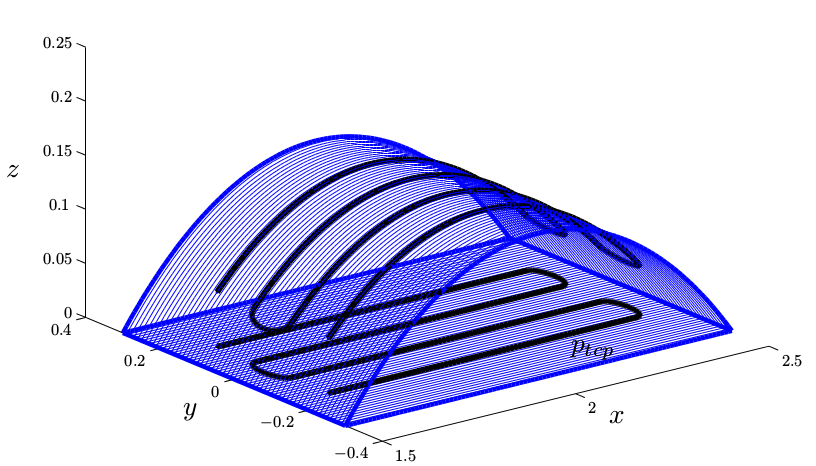
\includegraphics[width=.5\columnwidth]{figs/planejamento/pal.png}
	\caption{Subregiões de uma superfície.}
	\label{fig::pal}
\end{figure}


A superfície descrita na seção~\ref{modelagem} é uma equação implícita, na forma
$f(x,y,z)=0$. Neste caso, as trajetórias a serem percorridas pelo manipulador
podem ser obtidas através da interseção (cortes) entre planos uniformemente
espaçados e a superfície, o que gerará curvas ao longo da superfície. Uma ideia
semelhante e propícia devido à geometria do rotor, é gerar as curvas a partir da interseção
entre esferas e a superfície. As figuras~\ref{fig::interfrontal}
e~\ref{fig::interiso} mostram duas visões de duas interseções entre esferas e
a pá, onde as interseções estão representadas em vermelho.. Os mesmos cortes
podem ser observados entre esferas e o modelo algébrico da pá, em figura~\ref{fig::intergeo}.


\begin{figure}[t!]
	\centering
	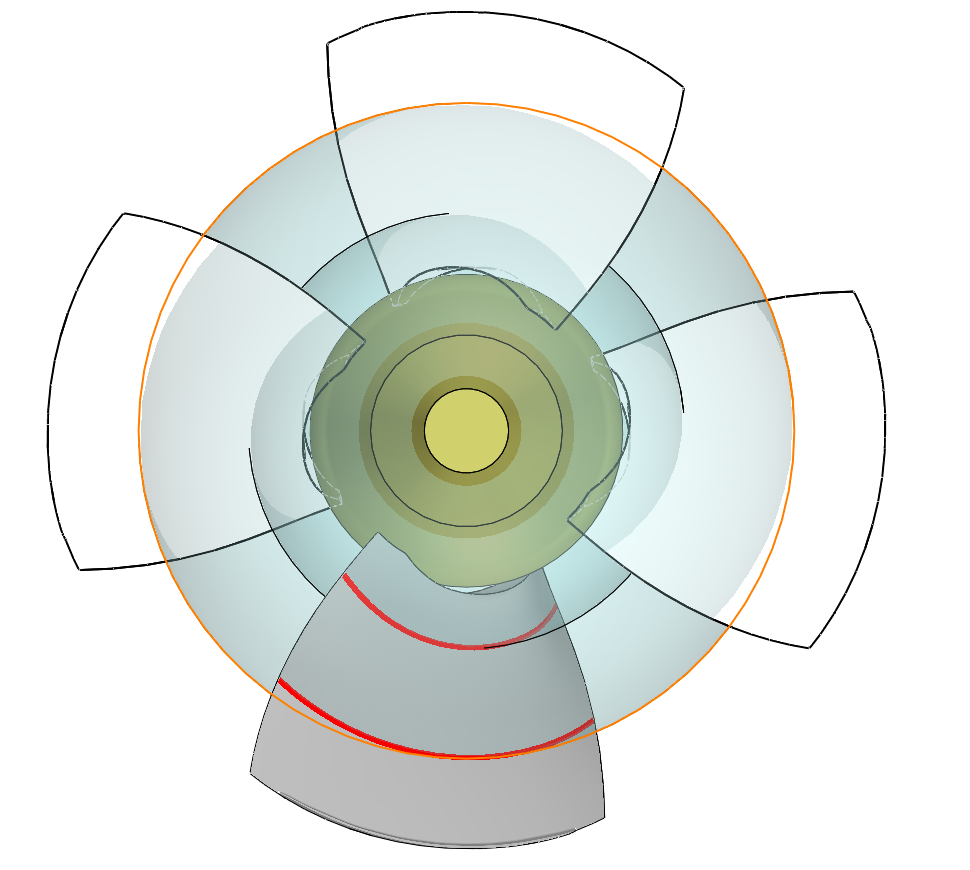
\includegraphics[width=0.5\columnwidth]{figs/planejamento/intersecao_frontal.PNG}
	\caption{Interseção esfera-pá, vista frontal.}
	\label{fig::interfrontal}
\end{figure}

\begin{figure}[t!]
	\centering
	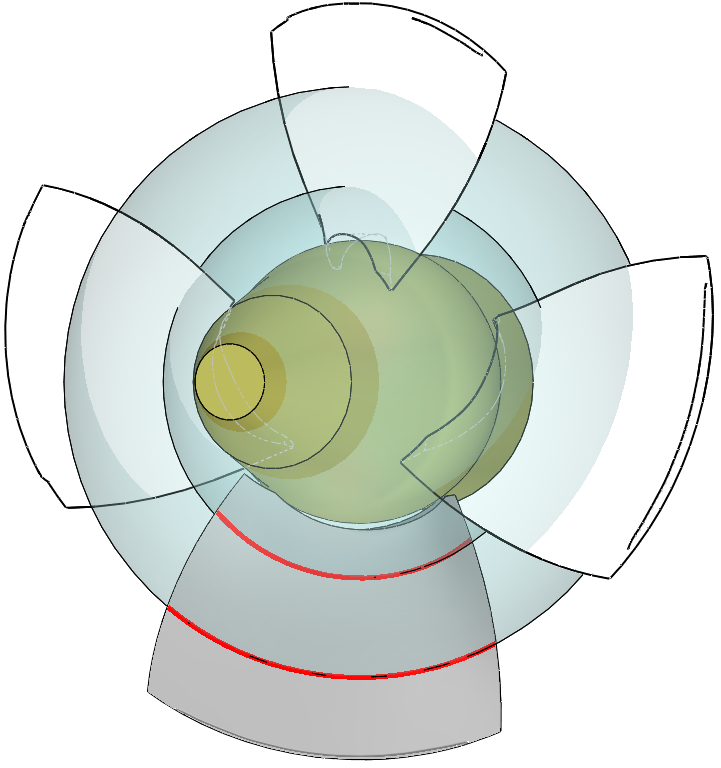
\includegraphics[width=0.5\columnwidth]{figs/planejamento/intersecao_iso.PNG}
	\caption{Interseção esfera-pá, vista isométrica.}
	\label{fig::interiso}
\end{figure}

\begin{figure}[t!]
	\centering
	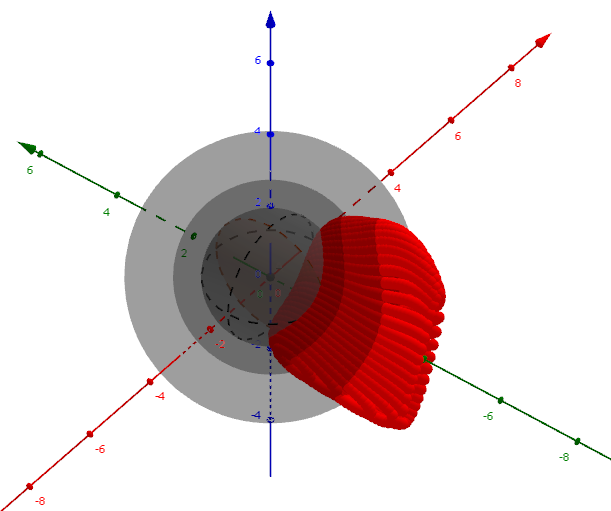
\includegraphics[width=0.5\columnwidth]{figs/planejamento/intersecao_geogebra.png}
	\caption{Interseção esfera-modelo pá.}
	\label{fig::intergeo}
\end{figure}


\subsubsection{Definição de caminho}
% Como transitar entre as paralelas de forma contínua